\documentclass[10pt,twocolumn]{article}
\usepackage{iasted}
\usepackage{floatflt}

\usepackage{times}
%\usepackage[dvips]{graphicx}
\usepackage[pdftex]{graphicx}

%\setlength{\intextsep}{0.2cm}
%\setlength{\dbltextfloatsep}{-0.5cm}
%\setlength{\textfloatsep}{-0.5cm}
%\setlength{\belowcaptionskip}{-0.5cm}

\begin{document}

\date{}

\title{BENCHMARKING TOOLS FOR FAIRLY COMPARING WATERMARKING ALGORITHMS}

\author{Stewart I. Fraser \\
        Department of Engineering \\
        University of Aberdeen \\
        Aberdeen, AB24 3UE, UK \\
	%Tel: +44 1224 273830 \\
	%Fax: +44 1224 272497 \\
        Email: s.i.fraser@abdn.ac.uk 
        \and
        Alastair R. Allen \\
        Department of Engineering \\
        University of Aberdeen \\
        Aberdeen, AB24 3UE, UK \\
	%Tel: +44 1224 272501 \\
	%Fax: +44 1224 272497 \\
        Email: a.allen@abdn.ac.uk
}

\addtolength{\parskip}{0.4cm}

\maketitle
\thispagestyle{empty}

%%%% Replace with your abstract.
\noindent
{\bf\normalsize ABSTRACT}\newline {
Fair benchmarking tools for comparing watermarking systems are introduced.
Three different watermarking systems 
are fairly compared using these tools. 
%using these benchmarking tools.
%(spatial, Discrete Cosine Transform (DCT) and 
%Discrete Wavelet Transform (DWT) based) 
%Watermarks are inserted into different greyscale digital images using these systems. 
The parametric values for each watermarking system
are carefully selected so
that the resultant watermarked images all have equal measures of visual degradation. 
The Watson Metric, which is based upon the Human Visual System (HVS), is used to compute the visual degradation.
The watermarked images are subjected to signal processing attacks. 
The robustness of each watermarking system is analysed using the fair benchmarking tools.
The effect of adding Error Correcting Codes (ECC) to these watermarking systems is also studied. 
Using fair benchmarking tools, it is shown that, in certain cases, what appears to be an increase in robustness is 
in fact a decrease in robustness.
}
\vspace{2ex}


%%%% Replace with your keywords. 
\noindent
{\bf\normalsize KEY WORDS}\newline
{Watermarking Techniques, Digital Image Watermarking, Benchmarking.}

\section{Introduction}
The need to provide copyright protection to digital media is of great importance in today's connected world.
This may be attributed to the widespread use of the internet which allows users to download perfect
copies of digital media onto their computers. In order to combat this problem, various watermarking systems
have been developed which allow 
authors of digital media to protect their
copyrighted works. 

There are many issues to consider when inserting a watermark for copyright protection, for example: (1) type of host image, (2) length of watermark,
(3) type of watermark (e.g., one-bit watermark or binary payload watermark), (4) embedding strength, (5) 
attacks that the watermark is likely to undergo. All of these issues will have a bearing upon the robustness of
a watermarking system.
%as well as determining which, if any, ECC scheme would best improve robustness.

In \cite{ECCb4:book, petit99}, methodologies for fairly comparing different
watermarking systems were outlined. 
It was suggested that the following attributes be measured: (1) visual degradation caused by the watermark,
(2) robustness of the watermarking system to attack and (3) the reliability of system.
In a watermarking system, there is a trade off between robustness and watermark perceptibility. Thus, for fair
evaluation and comparison of different systems, the parameters of each system need to be set so that the resultant
marked images have equal amounts of visual degradation. In this paper, the visual degradation is measured
using the Watson Metric~\cite{watson1Pap, watson2Pap, volo2nd}. This metric is based upon the Human
Visual System (HVS); thus, it is better than the pixel based Peak Signal to Noise Ratio (PSNR) metric.
The robustness of the different watermarking systems is measured by computing the Normalised Correlation (NC)
between the original and recovered watermarks.
To ensure statistically valid results, many tests are run using different watermarks and different insertion keys.
Performing these steps ensures a fair and unbiased comparison of the different watermarking systems.

The reliability of the watermarking systems under test was computed using Receiver Operating Characteristic (ROC) graphs. 
ROC graphs~\cite{rocErk98}
% rocErk98} 
%rocChak92}
are very useful in assessing the overall behaviour and reliability of a watermarking system.
Fair detector thresholds were set using Probability of False Positive ($P_{\mathit fp}$) calculations~\cite{kundurPfp}. 
By considering $P_{\mathit fp}$ while computing detector thresholds, the chance of obtaining a \emph{false positive}
reading for watermark presence becomes statistically unlikely. 

This work was extended by adding Error Correcting Codes (ECC) to the watermarking systems under investigation. 
Many authors \cite{marvelPap, 
wangPap, 
herrPap, 
%langPap, 
egg1Pap} 
%th4Pap, th5Pap}
have stipulated that various forms of ECCs have been incorporated
into their watermarking systems in order to increase robustness. 
%These include Bose, Chaudhuri and Hocquenghem (BCH) codes, Reed-Solomon codes, Hamming codes and Turbo codes.
However, many of these authors
do not compare the performance of watermarks with ECCs against watermarks without ECCs. This may lead
one to believe that adding ECC to a watermarking system will automatically result in better performance. 
To this end, Bose, Chaudhuri and Hocquenghem (BCH) codes~\cite{BKX:bchPlessBk} 
%bchLin} 
were added to the watermarking systems under investigation and their effect 
studied.


\section{Methodology}
\label{sec:meth}
%\subsection{The watermarking systems}
A fair comparison of three different watermarking systems was carried out.
These comprised the spatially based Bruyndonckx \emph{et al.}~\cite{bruyn1Pap} watermarking system, 
the Discrete Cosine Transform (DCT) based Koch \emph{et al.}~\cite{koch1Pap} system, and 
the Discrete Wavelet Transform (DWT) based Xie \emph{et al.}~\cite{xiePap} system.  All three of these systems are blind, each embed a binary watermark within the 
host image and it is the goal of all three to provide copyright protection.
%The code for these three watermarking systems can be obtained from \cite{meerwaldPap}.

The Bruyndonckx algorithm works in the spatial domain and selects non-overlapping blocks of $8 \times 8$. Elementary 
perceptual calculations are performed in these blocks by classifying pixels into zones of homogeneous luminance. One
bit of a binary watermark $\in\{0,1\}$ is embedded in the relationship between mean values in these zones of homogeneous 
luminance.

The Koch algorithm takes the DCT of non-overlapping $8 \times 8$ blocks. Two random DCT coefficients from the middle frequency range
are selected. The relationship between these two coefficients is altered to encode a binary watermark $\in\{0,1\}$.

The Xie algorithm runs a non-overlapping $1 \times 3$ window across the low frequency sub-band of the DWT. The coefficients in
these windows are sorted and the median value is quantised to represent a watermark bit $\in\{0,1\}$.

\subsection{The Watson metric}
The three watermarking systems were fairly compared by setting their parametric values so that
the marked images that they produced were of equal visual degradation. This visual degradation was
quantitatively measured using the Total Perceptual Error (TPE) measurement calculated from the 
Watson Metric \cite{watson1Pap}. 
The Watson Metric is based upon the Human Visual System (HVS).
This makes it a better quality metric than the commonly used Peak Signal to Noise Ratio (PSNR) metric which merely measures the pixel based
difference between the original and the watermarked image (it does not take the HVS into consideration).
The Watson metric weights the errors for each DCT coefficient in each block by its corresponding sensitivity threshold
(which is a function of contrast sensitivity, luminance masking and contrast masking). 
%The {\bf contrast sensitivity} 
%returns a visibility threshold for a given DCT component, the parameters of which were developed via extensive tests and are
%now widely adopted. 
%{\bf Luminance masking} accounts for the interaction between lumiance and frequency:
%\begin{equation}
%t_{ijk}=t_{ij}\left( \frac{c_{00k}}{\overline{c}_{00}} \right)^{a_{t}}
%\end{equation}
%where $c_{00k}$ is the DC coefficient of block $k$, $\overline{c}_{00}$ is the
%mean luminance of the display and $a_{t}$ determines
%the degree of masking (typically set to 0.65).
%{\bf Contrast masking} refers to the fact that the visibility of a pattern is reduced by the presence of another pattern in the image.
%This masking is strongest when both components are of the same spatial frequency, orientation and location:
%\begin{equation}
%m_{ijk}=\mbox{max}\left[t_{ijk}, \left|c_{ijk}\right|^{w_{ij}} {t_{ijk}}^{1-w_{ij}}\right]
%\end{equation}
%where $m_{ijk}$ is the masked threshold and $w_{ij}$ determines the degree of
%contrast masking. Typically $w_{00}=0$ and, 
%for all other coefficients, 
%$w_{ij}=0.7$. 
%The {\bf perceptual error} in each frequency of each block may be expressed as:
%\begin{equation}
%d_{ijk}=\frac{e_{ijk}}{m_{ijk}}
%\end{equation}
%where $e_{ijk}$ is the quantization error. To get the {\bf Total Perceptual Error (TPE)} independent
%of the image size, errors are pooled over space and frequency via the formula:
%\begin{equation}
%\label{eqn:tpePool}
%TPE = \frac{1}{N^{2}} \sum_{k} \sum_{i,j} \left|d_{ijk}\right|.
%\end{equation}
The higher the TPE value, the more the image has been degraded.
A more detailed 
%mathematical 
description of the Watson Metric can be found in \cite{watson2Pap, volo2nd}.

\subsection{BCH codes}
%Two different lengths of watermark, consisting of 80 and 320 bits, were tested. 
%For the 80 bit watermark, 
The following BCH~\cite{BKX:bchPlessBk} 
%bchLin} 
coding strategies were used:
BCH(80,52,9), BCH(80,38,13), BCH(80,24,19), 
BCH(320,203,27), BCH(320,113,51), BCH(320,24,79)
as well as the uncoded case. The BCH codes are in the form of BCH(\emph{n},\emph{k},\emph{d}),
where \emph{n} is the total length (\emph{i.e.}, the watermark), \emph{k} is the length of the message (that the user wishes to embed) 
and \emph{d} is the minimum distance. A BCH code can correct up to \emph{t} errors, where $d = 2t + 1$.
%For the 320 bit watermarks, the following BCH coding strategies were used:
%(320,257,15), (320,203,27), (320,158,39), (320,113,51), (320,68,61), (320,29,79)
%as well as the uncoded case.

\subsection{Signal processing attack}
\label{sec:SPatt}
Watermarking systems which attempt to provide copyright protection must be resilient
to different forms of attack. Such attacks include, amongst others, compression, noise addition, filtering,
cropping, resizing and rotation. 
These attacks can be grouped into two categories: (1) signal processing
attacks and (2) geometrical attacks. Signal processing attacks (\emph{e.g.} noise addition,
compression and filtering) reduce
watermark energy within an image. After such an attack, a decoder can locate
the pixels that have been marked but it cannot necessarily detect the watermark correctly
(due to the low energy of the watermark).
Geometrical attacks (\emph{e.g.} cropping, resizing and rotation) attempt to desynchronize
the watermark at the decoder. When desynchronization occurs, the decoder cannot find the
pixels that have been marked and thus cannot detect the watermark.
This paper focuses upon signal processing attacks only. 
%(assuming geometrical attacks have been resynchronized at the decoder).
%For desychronization attacks, such
%as cropping and resizing, it is assummed that the decoder has successfully
%resychronized with the watermark after compensating for geometrical distortions.
A more detailed discussion of geometrical attacks and resynchronization techniques can be found in
\cite{
%tpunRST1, 
tpunRST2, 
%tpunRST3, 
%tpunRST4, 
%wangRST, 
linRST, 
%senRST, 
%ozerRST, 
patrickBasRST, 
%ECCb4:volo,
voloGreece2001}.
%ECCb4:volo
The signal processing attack of JPEG compression is used in this paper.

%Five different greyscale $256\times 256$ host images, each widely used in the image processing literature, were used to embed
%the watermarks. Each of the watermarking systems under test was then attacked with the signal processing attack of
%JPEG\footnote{the 
%\emph{imwrite} function (from MATLAB 6, Release 12) was used}
%compression; 
%the JPEG strengths varied, from 10\% quality to 100\% quality, in steps of 5\%. 
%Each JPEG attack was performed fifty times each and then averaged. Each time, a different key and different binary watermark were used.
%JPEG compression was chosen for the attack as it is one of the most widely used still image compression schemes.
%The \emph{imwrite} function (from MATLAB 6, Release 12) was used
%to JPEG compress the watermarked images. The \emph{imwrite} function uses the Independent JPEG Group's (www.ijg.org) LIBJPEG library.

\subsection{Measuring robustness}
\label{sec:robust}
Each JPEG quality attack level was performed fifty times upon each host image. 
This was repeated for all three watermarking systems under test.
%for each of the three algorithms under test. 
For each JPEG quality attack level, a different seed value and a
different binary watermark $\in\{0,1\}$ were embedded into the test image.  For all fifty attacks, the original 
and recovered messages were compared by computing the Normalised Correlation (NC):
\begin{equation}
	\mbox{NC}= \frac {m^{*} \cdot m} {||m^{*}|| \cdot ||m||}
\end{equation}
where $m$ is the original message and $m^{*}$ is the recovered message (convert unipolar vectors, $m\in\{0,1\}$, to
bipolar vectors, $m\in\{-1,1\}$, in this equation).
These fifty NC values were averaged, resulting in a single NC value for a particular JPEG quality level in a particular image for a 
specific watermarking system. A graph of NC against JPEG quality was plotted for each watermarking system and each host image.
%The MATLAB code for calculating the NC between two binary vectors is shown below:
%
%\footnotesize
%%\renewcommand{\baselinestretch}{1}
%\begin{verbatim}
%function theNC = NCcalc(embeddedWM,recoveredWM);
%theCorr = 0;
%for i=1:length(embeddedWM)
%    if recoveredWM(i) == embeddedWM(i)
%        corr = corr + 1;
%    else
%        corr = corr - 1;
%    end
%end; clear i;
%theNC = corr / length(embeddedWM);
%\end{verbatim}
%%\renewcommand{\baselinestretch}{1.5}
%\normalsize

\subsection{Probability of false positives}
Different detector thresholds are calculated for different message lengths that result in Probability of False Positive
($P_{\mathit fp}$) 
values of similar magnitude.
These detector threshold values are then used to fairly analyse the NC against JPEG quality graphs 
for different message lengths.
As described in \cite{kundurPfp}, the $P_{fp}$ for a binary vector can be calculated via:
\begin{equation}
\label{eq:Pfp}
        P_{fp} = \sum^{N_{w}}_{n= \lceil N_{w}(T+1)/2 \rceil} \left(
                                                                        \begin{array}{c}
                                                                                N_{w} \\
                                                                                n
                                                                        \end{array}
                                                              \right)                           0.5^{N_{w}}
\end{equation}
where $N_{w}$ is the message length, $T$ is the chosen detector threshold and:
\begin{equation} 
\label{eq:PfpBKX_2}
								\left(
                                                                        \begin{array}{c}
                                                                                N_{w} \\
                                                                                n
                                                                        \end{array}
                                                              	\right)				=  	\frac{N_{w}!}{n!(N_{w}-n)!}.
\end{equation} 
%$
%								\left( 
%                                                                       \begin{array}{c}
%                                                                                N_{w} \\
%                                                                                n
%                                                                        \end{array}
%                                                             	\right)				=  	\frac{N_{w}!}{n!(N_{w}-n)!}.
%$
%The MATLAB code used to determine a $P_{fp}$ reading is shown below:
%\footnotesize
%%\renewcommand{\baselinestretch}{1}
%\begin{verbatim}
%function Pfp = falsePosCalc(T,Nw);
%n = floor(Nw*(T+1)/2);
%Pfp = 0.0;
%for i = n:Nw
%    factVal = factorial(Nw) / ...
%         (factorial(i) * factorial(Nw-i));
%    Pfp = Pfp + (factVal * (0.5 ^ Nw));
%end; clear i;
%\end{verbatim}
%%\renewcommand{\baselinestretch}{1.5}
%\normalsize

\subsection{ROC graphs}
%In any watermarking system, the detector has to decide whether an image has been watermarked
%or whether it has not been watermarked~\cite{ECCb4:book}. This is an example of binary hypothesis testing in that
%the decoder has to choose between two opposing possibilities. 
%These two opposing possibilities are the null hypothesis
%(the image does not contain the watermark) and the alternative hypothesis (the image 
%does contain the watermark). 
%In hypothesis testing, a threshold is set and a test statistic is 
%compared to this threshold in order to select either the alternative hypothesis
%or the null hypothesis. 
%In the case of watermarking, the test statistic is the normalised correlation between the embedded and
%recovered watermarks. The alternative hypothesis is the presence of the watermark and the 
%null hypothesis is the absence of the watermark.
Comparing different watermarking systems using a fixed threshold for the normalised correlation
measurement 
%(in order to decide between the alternative hypothesis and the null hypothesis) 
could give misleading results
(especially if the visual degradations had not been set equal nor $P_{\mathit fp}$ calculations considered)~\cite{ECCb4:book}.
Different watermarking systems have very different \emph{modis operandi} and as such it is not prudent 
to set the same threshold value for every watermark detector. A more sensible approach is to 
treat each watermarking system as a separate entity and calculate an individual threshold value
for each detector. 
ROC graphs~\cite{rocErk98} 
%rocErk98} 
%rocChak92}
address this problem by continuously varying the threshold over 
a wide range of values. This has the benefit of giving a fair comparison of
watermarking systems that have very different embedding/detection methods.
The performance of the detector can be quantified by calculating the area\footnote{done using the MATLAB \emph{trapz} function}
beneath the 
ROC curve.
For an ideal detector, the area would be 1.00. For a worthless detector (a detector
that randomly selects if an image is watermarked or not),
the area would be 0.50.






\section{Results: 80 bit watermarks}
Results for 80 bit watermarks are presented. The 80 bit watermarks consist of the following:
(1) uncoded 80 bit message, (2) BCH(80,52,9): message of 52 bits with 28 ECC bits, can correct 4 errors,
(3) BCH(80,38,13): message of 38 bits with 42 ECC bits, can correct 6 errors, (4) BCH(80,24,19): message
of 24 bits, 56 ECC bits, can correct 9 errors. 
Three different greyscale images, each $256\times256$, are used as hosts for the watermarks.
These are the Pentagon image, the Fishingboat image and the Lena image (each widely used in image processing
literature). The watermarked images are attacked with JPEG compression (a signal processing attack, see Section~\ref{sec:SPatt}).
Graphs of NC against JPEG quality are plotted for each watermarking system and each host image.
The parameters for all three watermarking systems are chosen so that the resultant TPEs, measured via
the Watson Metric (block size of $8\times8$), are all 0.002. This value indicates that the watermarks
are imperceptible to a human viewer. 

Table~\ref{bkxVQBKX} shows the embedding strengths used for each algorithm and
the resulting visual degradations. 
\begin{table}[!htb]
%\small
\footnotesize
        \begin{center}
                \begin{tabular}{|c|c|c|c|c|} \hline
				& 		 & PSNR		&      	& Embedding   	\\	
                Algorithm	&Image           & (dB)     	& TPE  	& strength    	\\ \hline \hline
                %Bruyndonckx	&Baboon          & 46.07        & 0.002	& 7.50          \\ \cline{2-5}
                Bruyndonckx	&Lena            & 46.75        & 0.002	& 7.50          \\ \cline{2-5}
                %		&Peppers         & 45.09        & 0.002	& 7.50          \\ \cline{2-5} \hline\hline 
                		&Fishingboat     & 46.18        & 0.002	& 7.50          \\ \cline{2-5}
                		&Pentagon        & 46.83        & 0.002	& 7.50          \\ \hline\hline
		%Koch		 &Baboon          & 42.89       & 0.002 & 5.00         \\ \cline{2-5}
                Koch		&Lena            & 43.59        & 0.002 & 5.00          \\ \cline{2-5}
                %		&Peppers         & 43.95        & 0.002 & 7.50          \\ \cline{2-5} \hline\hline
                \scriptsize\emph{(JPEG quality}\normalsize	
				&Fishingboat     & 43.05        & 0.002 & 7.50          \\ \cline{2-5}
                \scriptsize\emph{setting of 90)}\normalsize		
				&Pentagon        & 42.12        & 0.002 & 7.50          \\ \hline\hline
		%Xie		 &Baboon          & 50.02       & 0.002 & 0.11         \\ \cline{2-5}
                Xie		&Lena            & 48.81        & 0.002 & 0.10          \\ \cline{2-5}
                %		&Peppers         & 47.99        & 0.002 & 0.11          \\ \cline{2-5} \hline
                \scriptsize\emph{(4 wavelet levels)}\normalsize	
				&Fishingboat     & 47.29        & 0.002 & 0.18          \\ \cline{2-5}
                		&Pentagon        & 50.55        & 0.002 & 0.25          \\ \hline
                \end{tabular}
		\caption{Visual quality of 
			images with 80 bit watermarks} 
                \label{bkxVQBKX}
        \end{center}
\end{table}
As was suggested in~\cite{petit99}, it is safe to assume that a binary watermark
is detected if 80\% of the bits match the original. This is equivalent to a NC value of 0.60. For a binary vector
of length 80 bits, the probability of randomly obtaining a false positive reading when using a detector threshold
value of 0.60 is is $2.5 \times 10^{-8}$ (equation \ref{eq:Pfp}). Thus, for message lengths of 52, 38 and 24, detector
thresholds are chosen that result in $P_{\mathit fp}$ values of similar magnitude. These detector threshold values and
their corresponding $P_{\mathit fp}$ values are shown in Table~\ref{tab:80ResBKX}.
\begin{table}[!htb]
\footnotesize
        \begin{center}
		\begin{tabular}{|c|c|c|c|} \hline
				& Coding		& Detector	& 		\\ 
		Algorithm 	& strategy		& threshold	& $P_{fp}$ 	\\\hline\hline

		Bruyndonckx	& uncoded		& 0.60		& \raisebox{-0.3ex}{ $2.5\times 10^{-8}$ }	\\ \cline{2-4}
				& BCH(80,52,9)		& 0.75		& \raisebox{-0.4ex}{ $3.5\times 10^{-8}$ }	\\ \cline{2-4}
				& BCH(80,38,13)		& 0.85		& \raisebox{-0.4ex}{ $3.3\times 10^{-8}$ }	\\ \cline{2-4}
				& BCH(80,24,19)		& 1.00		& \raisebox{-0.4ex}{ $6.0\times 10^{-8}$ }	\\ \hline\hline

		Koch 		& uncoded		& 0.60		& \raisebox{-0.3ex}{ $2.5\times 10^{-8}$ }	\\ \cline{2-4}
				& BCH(80,52,9)		& 0.75		& \raisebox{-0.4ex}{ $3.5\times 10^{-8}$ }	\\ \cline{2-4}
				& BCH(80,38,13)   	& 0.85  	& \raisebox{-0.4ex}{ $3.3\times 10^{-8}$ }	\\ \cline{2-4}	
				& BCH(80,24,19)		& 1.00		& \raisebox{-0.4ex}{ $6.0\times 10^{-8}$ }	\\ \hline\hline	

		Xie		& uncoded               & 0.60		& \raisebox{-0.3ex}{ $2.5\times 10^{-8}$ }	\\ \cline{2-4}
				& BCH(80,52,9)          & 0.75		& \raisebox{-0.4ex}{ $3.5\times 10^{-8}$ }	\\ \cline{2-4} 	
				& BCH(80,38,13)         & 0.85 		& \raisebox{-0.4ex}{ $3.3\times 10^{-8}$ }	\\ \cline{2-4} 
				& BCH(80,24,19)         & 1.00		& \raisebox{-0.4ex}{ $6.0\times 10^{-8}$ }	\\ \hline 
	\end{tabular} 
	\caption{Detector thresholds for different message lengths}
	\label{tab:80ResBKX}
	\end{center}
\end{table}
\normalsize
In Figure~\ref{fig:80BKX}, these different detector threshold values for different message lengths are represented by the
``thick'' horizontal lines at NC values of 0.60, 0.75, 0.85 and 1.00.
\begin{figure*}[!htb]
\setlength{\abovecaptionskip}{-0.25cm}
% ... original values, 7 aug 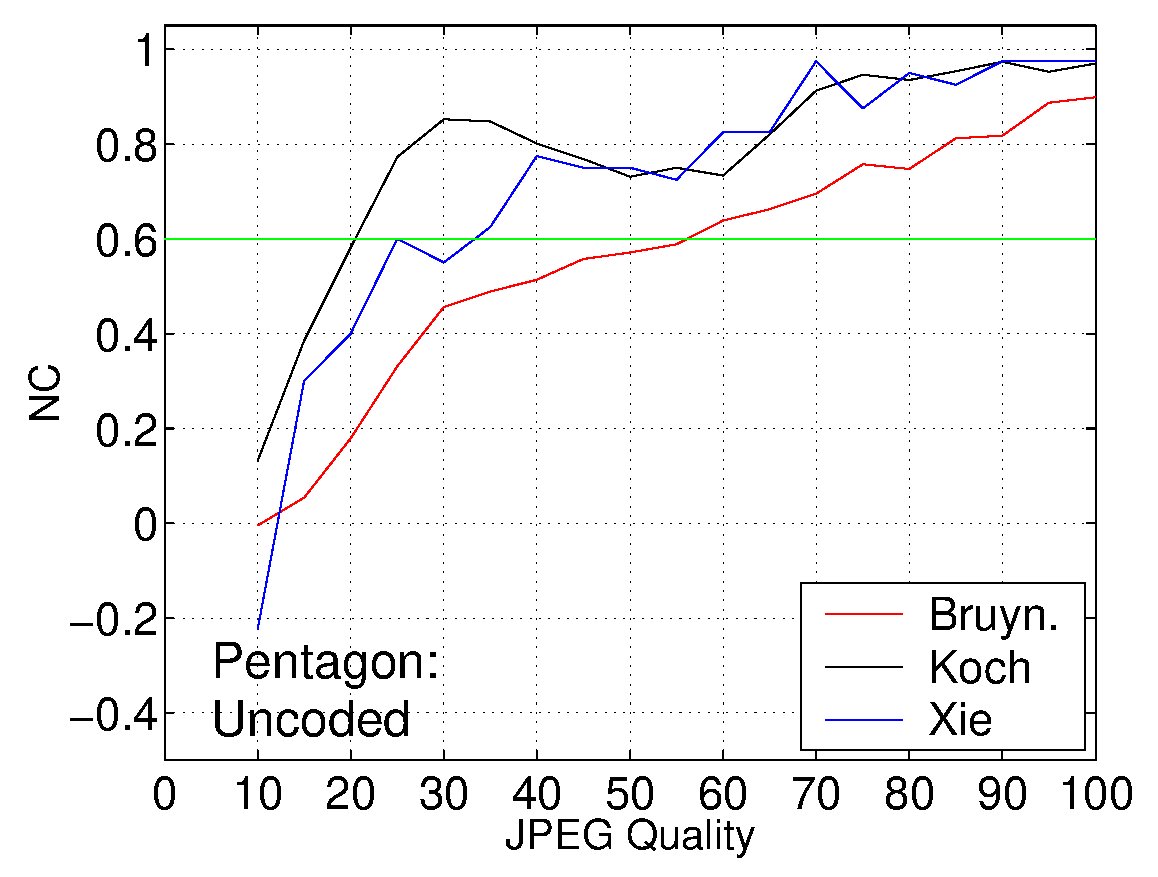
\includegraphics[height=4.6cm,width=4.8cm]{Pentagon80_80_1.eps}
\centerline{ \hbox{
        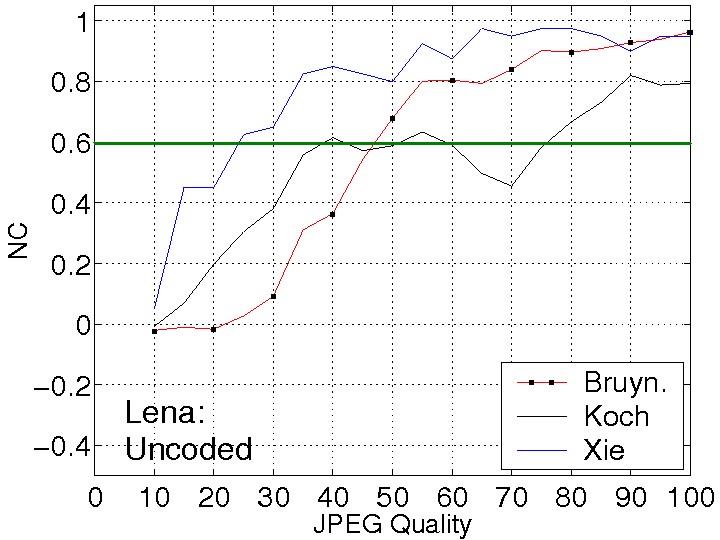
\includegraphics[height=4.5cm,width=4.5cm]{Lena80_80_1.png}
        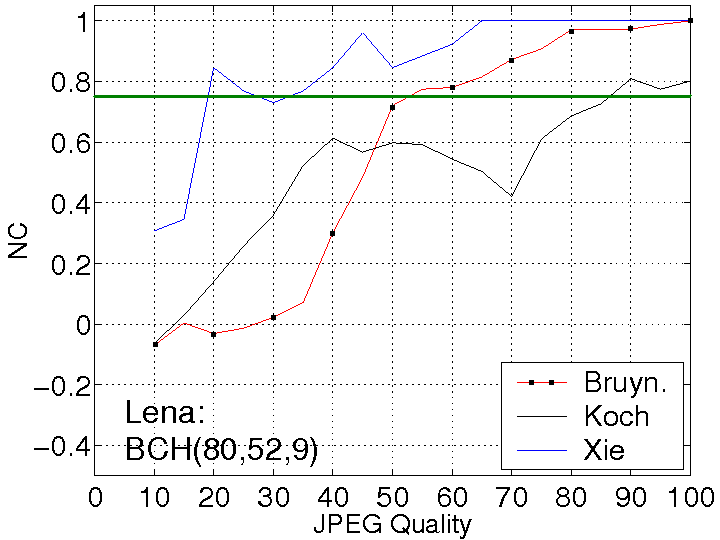
\includegraphics[height=4.5cm,width=4.5cm]{Lena80_52_9.png}
        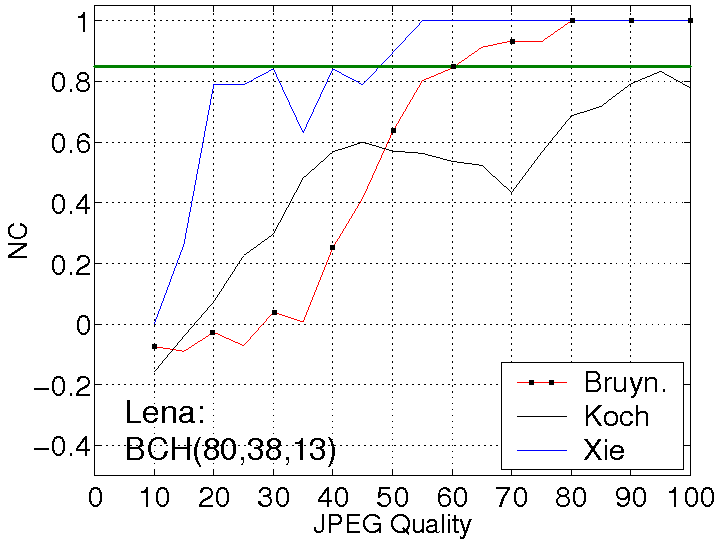
\includegraphics[height=4.5cm,width=4.5cm]{Lena80_38_13.png}
        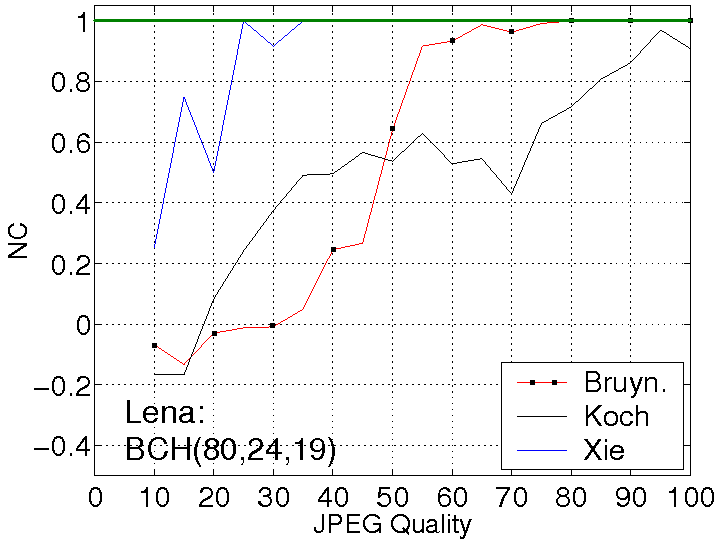
\includegraphics[height=4.5cm,width=4.5cm]{Lena80_24_19.png}
}} 
\centerline{ \hbox{
        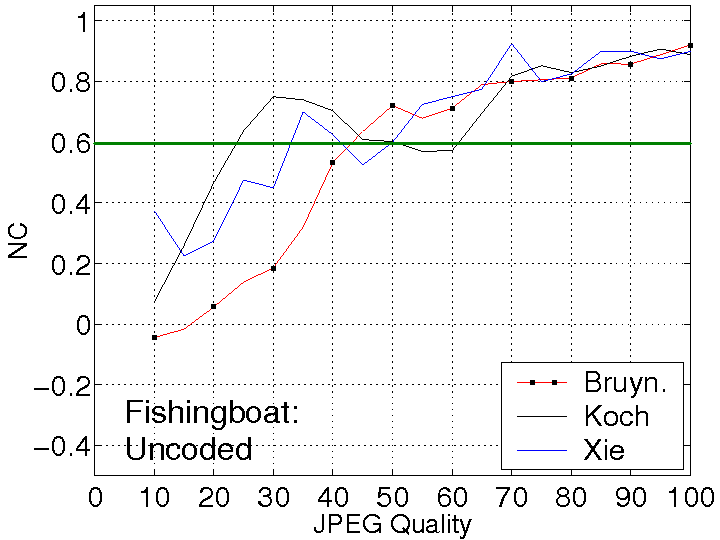
\includegraphics[height=4.5cm,width=4.5cm]{Fishingboat80_80_1.png}
        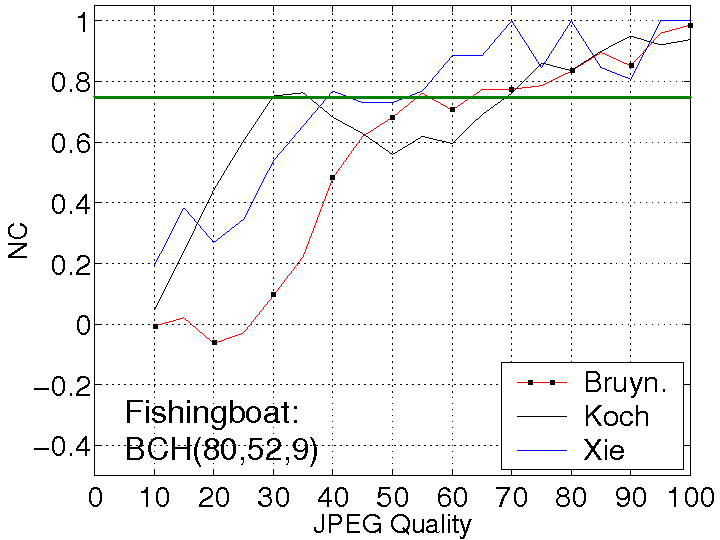
\includegraphics[height=4.5cm,width=4.5cm]{Fishingboat80_52_9.png}
        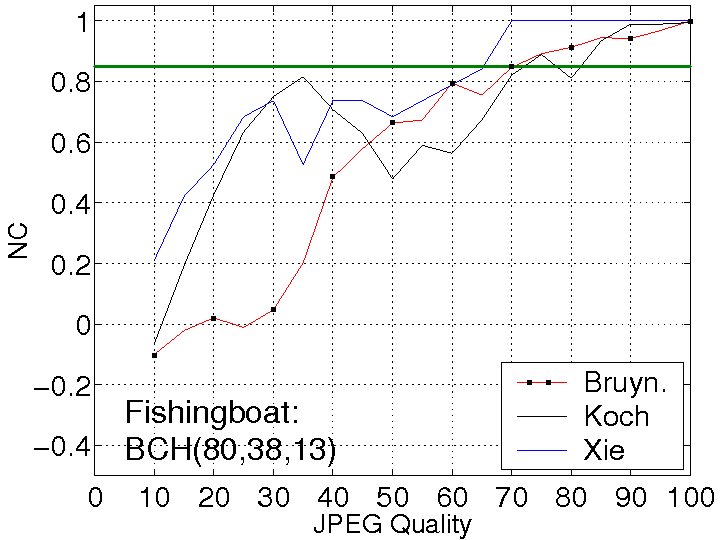
\includegraphics[height=4.5cm,width=4.5cm]{Fishingboat80_38_13.png}
        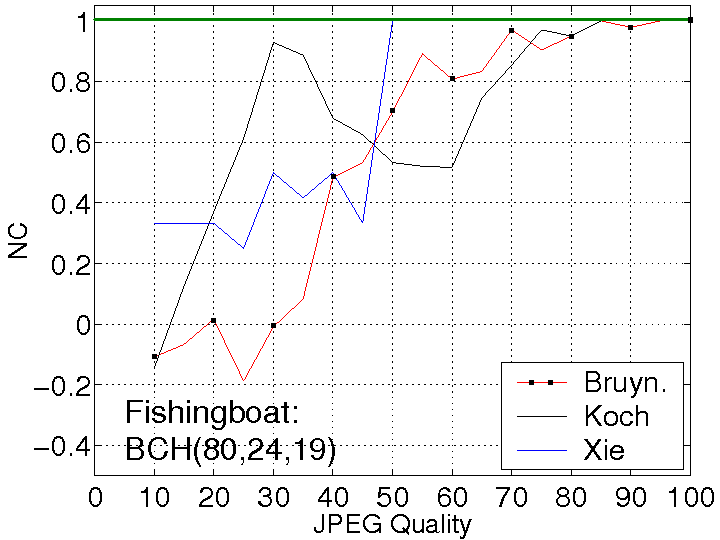
\includegraphics[height=4.5cm,width=4.5cm]{Fishingboat80_24_19.png}
}} 
\centerline{ \hbox{
        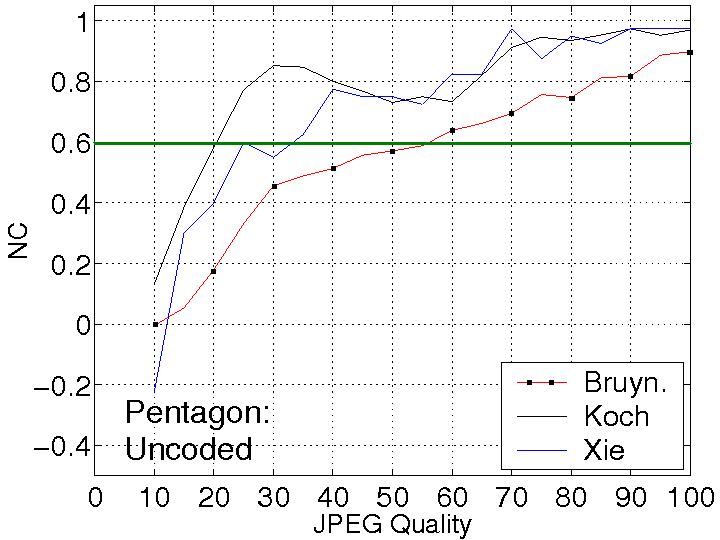
\includegraphics[height=4.5cm,width=4.5cm]{Pentagon80_80_1.png}
        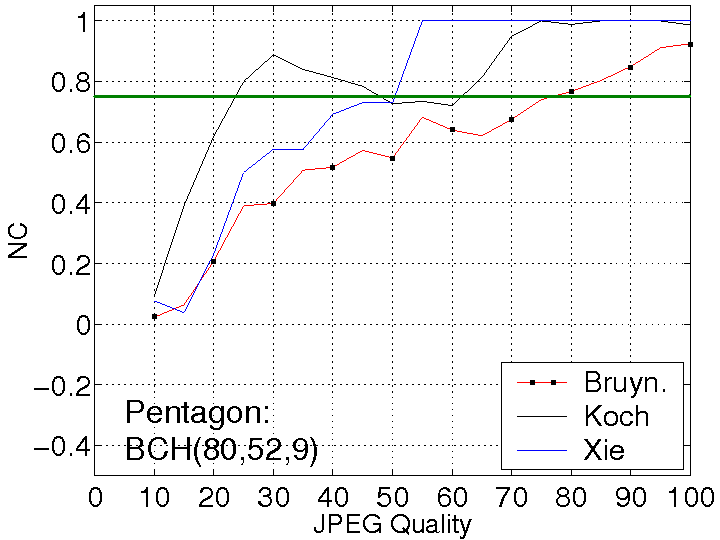
\includegraphics[height=4.5cm,width=4.5cm]{Pentagon80_52_9.png}
        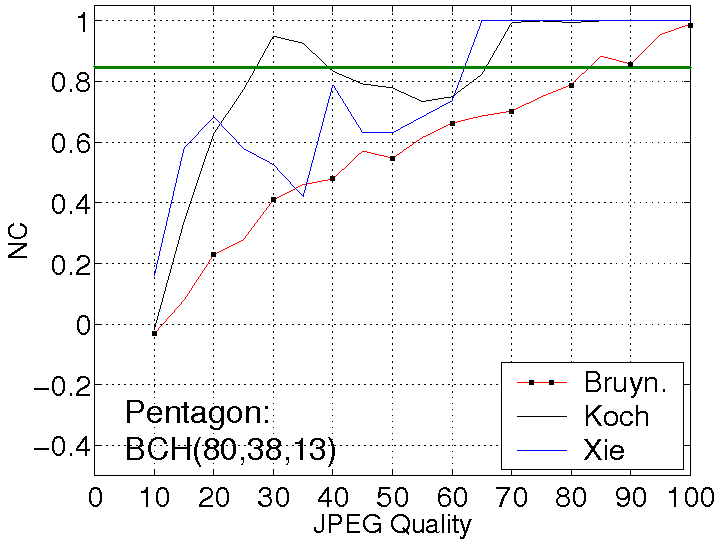
\includegraphics[height=4.5cm,width=4.5cm]{Pentagon80_38_13.png}
        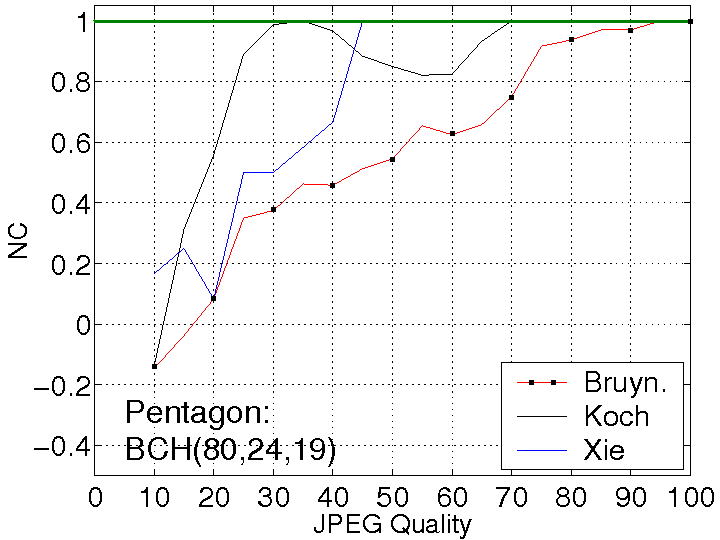
\includegraphics[height=4.5cm,width=4.5cm]{Pentagon80_24_19.png}
}} 
        \caption{Results for different watermarking systems using 80 bit watermarks}
        \label{fig:80BKX}
\setlength{\abovecaptionskip}{0cm}
\end{figure*}
Looking at the uncoded Lena graph in Figure~\ref{fig:80BKX} in 
conjunction with the detector thresholds in Table~\ref{tab:80ResBKX}, it can be seen that the Xie algorithm is the 
most robust. For all JPEG quality values 25 and greater, the Xie algorithm is returning
NC values greater than 0.60. The next most robust algorithm is the Bruyndonckx followed by the Koch algorithm. 
The Bruyndonckx algorithm is returning NC values greater than 0.60 for JPEG quality attacks of 50 and greater.
The Koch algorithm is returning NC values equal to or greater than 0.60 for JPEG quality attacks of 75 and greater.
Looking at the Lena:BCH(80,24,19) graph in Figure~\ref{fig:80BKX} (top right), the results are very different. Here, the 
Xie algorithm reaches the target NC of 1.00 at JPEG quality 35, the Bruyndonckx reaches NC of 1.00 at JPEG quality 80
and the Koch algorithm never reaches a NC value of 1.00. The two graphs between these two extremes, Lena:BCH(80,52,9)
and Lena:BCH(80,38,13), follow a pattern of the Xie algorithm being the most robust, then the Bruyndonckx algorithm and then
the Koch algorithm. It can be seen that the uncoded watermarks are performing the best; as more BCH coding is added,
the results deteriorate. 

The Bit Error Rate (BER) of this channel (watermarked image) is too high to reap the benefits of BCH coding
(with the watermark embedding strengths used in Table~\ref{bkxVQBKX}). 
The BER of the channel could be reduced by increasing the length of the watermark or embedding the watermark with
greater strength. However, both of these options would reduce the quality of the watermarked image.
It should be noted that as the level of BCH coding increases in the Lena image,
the NC values are increasing. However, because fair benchmarking tools have been used, it is clear that this is an \emph{apparent}
increase in robustenss only, the uncoded watermarks are performing better (although returning lower NC values).

Similar patterns of results are obtained for the Fishingboat and Pentagon images; as the level of BCH coding increases,
the performance of a particular watermarking system decreases. The image specific nature of watermarking systems can be
seen here too. In the Pentagon image, the Koch algorithm performs far stronger than it did in the Lena image. 
The Picture Information Measure (PIM)~\cite{BKX:shinPIM} 
%(PIM)~\cite{BKX:shinPIM, BKX:changPIM, mayacheDI}
can be used to ascertain the complexity of an image (the higher the PIM value of an image, the more inhomogeneous it is).
A PIM value is calculated for each $8\times8$ sub-block via:
\begin{equation}
	PIM = \left( \sum^{L-1}_{i=0}h(i) \right) - \mbox{max}_{i}[h(i)]
\end{equation}
where \emph{L} is the number of grey levels in a sub-block and \emph{h(i)} is a histogram for grey level \emph{i} in a sub-block.
%For example, a monotonous sub-block will have a small amount of highly populated bins, thus, $\mbox{max}_{i}[h(i)]$ will have 
%a large value and the PIM value will be small. A busy sub-block will have a uniformly distributed histogram (a large amount of
%poorly populated bins), thus, $\mbox{max}_{i}[h(i)]$ will be small and the PIM value will be large. Therefore, PIM measures the difference
%between the total number of pixels in a sub-block and the magnitude of the largest bin in the sub-block histogram.
The following PIM results were obtained: Lena (18848), Fishingboat (21513) and Pentagon (28442). It can be seen that 
Lena is the smoothest image, then Fishingboat and Pentagon is the busiest image. From this, it can be ascertained that 
the Xie and Bruyndonckx algorithms perform best in smooth images whereas the Koch algorithm performs best in busy images. 
Table \ref{bkzROCBKX} outlines the reliability of the watermarking systems via an analysis of the area under the ROC curves.
All systems can be said to be reliable as the areas under the curves are much closer to 1.00 than they are to 0.50.
Overall, it can be seen that the reliability of the transform based watermarking systems, Koch and Xie, are better (higher)
than that of the spatially based Bruyndonckx system. 
\section{Results: 320 bit watermarks}
The same three watermarking systems are tested again, however, watermarks of 320 bits are used rather than 80 bits.
The 320 bit watermarks consist of the following:
(1) uncoded 320 bit message, (2) BCH(320,203,27): message of 203 bits with 117 ECC bits, can correct 13 errors,
(3) BCH(320,113,51): message of 113 bits with 207 ECC bits, can correct 25 errors, (4) BCH(320,24,79): message
of 24 bits, 296 ECC bits, can correct 39 errors. 
\begin{table}[!ht]
%\footnotesize
\scriptsize
        \begin{center}
                \begin{tabular}{|c||c||c|c|c|c|} \hline
                           &                    & \multicolumn{4}{c|} {ROC Area}  \\ \cline{3-6}
                Algorithm &    Image           & \mbox{Uncoded} & BCH 		& BCH 		& BCH \\
			&			& 	& (80,52,9)	& (80,38,13)	& (80,24,19) \\ \hline \hline
                %Bruyn.&    Baboon          & 0.943 & 0.917 & 0.923 & 0.921 \\ \cline{2-6}
                Bruyn-  &       Pent.       & 0.938 & 0.946 & 0.923 & 0.890 \\ \cline{2-6}
                %       &       Peppers         & 0.884 & 0.833 & 0.826 & 0.819 \\ \cline{2-6}
                donckx  &       Fish.     & 0.883 & 0.845 & 0.832 & 0.811 \\ \cline{2-6}
                        &       Lena            & 0.862 & 0.832 & 0.780 & 0.804 \\ \hline\hline

                %Koch    &Baboon          & 0.990 & 0.981 & 0.964 & 0.953 \\ \cline{2-6}
                Koch     &Pent.       & 0.995 & 0.991 & 0.977 & 0.962 \\ \cline{2-6}
                %        &Peppers         & 0.987 & 0.970 & 0.960 & 0.929 \\ \cline{2-6}
                        &Fish.     & 0.990 & 0.982 & 0.973 & 0.950 \\ \cline{2-6}
                        &Lena            & 0.968 & 0.952 & 0.931 & 0.916 \\ \hline\hline

                %Xie     &               Baboon          & 0.971   & 0.966        & 0.914         & 0.957         \\ \cline{2-6}
                Xie     &               Pent.       & 0.933   & 0.913        & 0.893         & 0.927         \\ \cline{2-6}
                %        &               Peppers         & 0.958   & 0.998        & 0.994         & 0.952         \\ \cline{2-6}
                        &               Fish.     & 0.949   & 0.915        & 0.967         & 0.929         \\ \cline{2-6}
                        &               Lena            & 0.908   & 0.967        & 0.973         & 0.958         \\ \hline

                \end{tabular}
		%\caption{Area under ROC graphs over three different images watermarked using three different systems
		%with 80 bit watermarks under JPEG compression attack}
		\caption{Area under ROC graphs for 80 bit watermarks}
                \label{bkzROCBKX}
        \end{center}
\end{table}
%\end{table*}
\normalsize
Only the Lena image is used to embed the watermarks in these tests.
The parameters for the watermarking systems were set so that the TPE of all the 
watermarked images was 0.006. 
For this level of TPE, it is possible for a human viewer to note a difference when a watermarked image
is closely compared with an original image. Thus, the 320 bit watermarks have been inserted stronger
than the 80 bit watermarks.
Table~\ref{tab:3schemes320BKX}
shows the parametric values used in all the systems to produce watermarked images of equal degradation.
\begin{table}[!htb]
%\scriptsize
\footnotesize
        \begin{center}
                \begin{tabular}{|c|c|c|c|c|c|} \hline
				&		& Embedding	& Block		& JPEG 		& Wavelet \\
                Algorithm       & TPE           & strength    	& size    	& setting	& levels	 \\ \hline
                Bruyndonckx     & 0.006         & 7             & $8\times 8$   & -		& - 		\\ \hline
                Koch            & 0.006         & 5             & $8\times 8$   & 90		& - 		\\ \hline
                Xie             & 0.006         & 0.3           & $1\times 3$   & -		& 3 		\\ \hline
                \end{tabular}
		\caption{Visual quality of Lena with 320 bit watermarks}
                \label{tab:3schemes320BKX}
        \end{center}
\end{table}
\normalsize
Table~\ref{tab:320ResBKX} shows the detector thresholds chosen for each coding strategy that result in $P_{fp}$ values of
similar magnitude. From the graphs in Figure \ref{fig:320BKX}, it can be seen that the Xie algorithm is again the most robust
(in the Lena image). 
\begin{table}[!htb]
\footnotesize
        \begin{center}
		\begin{tabular}{|c|c|c|c|} \hline
				& Coding		& Detector	& 		\\ 
		Algorithm 	& strategy		& threshold	& $P_{fp}$ 	\\\hline\hline

		Bruyndonckx	& uncoded		& 0.40		& \raisebox{-0.3ex}{ $< 2.3\times 10^{-7}$ }	\\ \cline{2-4}
				& BCH(320,203,27)	& 0.40		& \raisebox{-0.4ex}{ $< 2.3\times 10^{-7}$ }	\\ \cline{2-4}
				& BCH(320,113,51)	& 0.50		& \raisebox{-0.4ex}{ $1.1\times 10^{-7}$ }	\\ \cline{2-4}
				& BCH(320,29,79)	& 0.90		& \raisebox{-0.4ex}{ $8.1\times 10^{-7}$ }	\\ \hline\hline

		Koch 		& uncoded		& 0.40		& \raisebox{-0.3ex}{ $< 2.3\times 10^{-7}$ }	\\ \cline{2-4}
				& BCH(320,203,27)	& 0.40		& \raisebox{-0.4ex}{ $< 2.3\times 10^{-7}$ }	\\ \cline{2-4}
				& BCH(320,113,51)   	& 0.50  	& \raisebox{-0.4ex}{ $1.1\times 10^{-7}$ }	\\ \cline{2-4}	
				& BCH(320,29,79)	& 0.90		& \raisebox{-0.4ex}{ $8.1\times 10^{-7}$ }	\\ \hline\hline	

		Xie		& uncoded               & 0.40		&  \raisebox{-0.3ex}{ $< 2.3\times 10^{-7}$ }	\\ \cline{2-4}
				& BCH(320,52,9)          & 0.40		&  \raisebox{-0.4ex}{ $< 2.3\times 10^{-7}$ }	\\ \cline{2-4} 	
				& BCH(320,38,13)         & 0.50 	& \raisebox{-0.4ex}{ $1.1\times 10^{-7}$ }	\\ \cline{2-4} 
				& BCH(320,24,79)         & 0.90		& \raisebox{-0.4ex}{ $8.1\times 10^{-7}$ }	\\ \hline 
	\end{tabular} 
	\caption{Detector thresholds for different message lengths}
	\label{tab:320ResBKX}
	\end{center}
\end{table}
\normalsize
In the {\bf Bruyndonckx system}, 
	the BCH decoded messages only improve on the uncoded 
	message NC values at high JPEG qualities (low compression rates).
	At low JPEG qualities, the performance of
	the BCH decoded messages is worse than the uncoded messages.
\begin{figure*}[!ht]
\setlength{\abovecaptionskip}{-0.25cm}
\centerline{ \hbox{
% ... original values, 7 aug 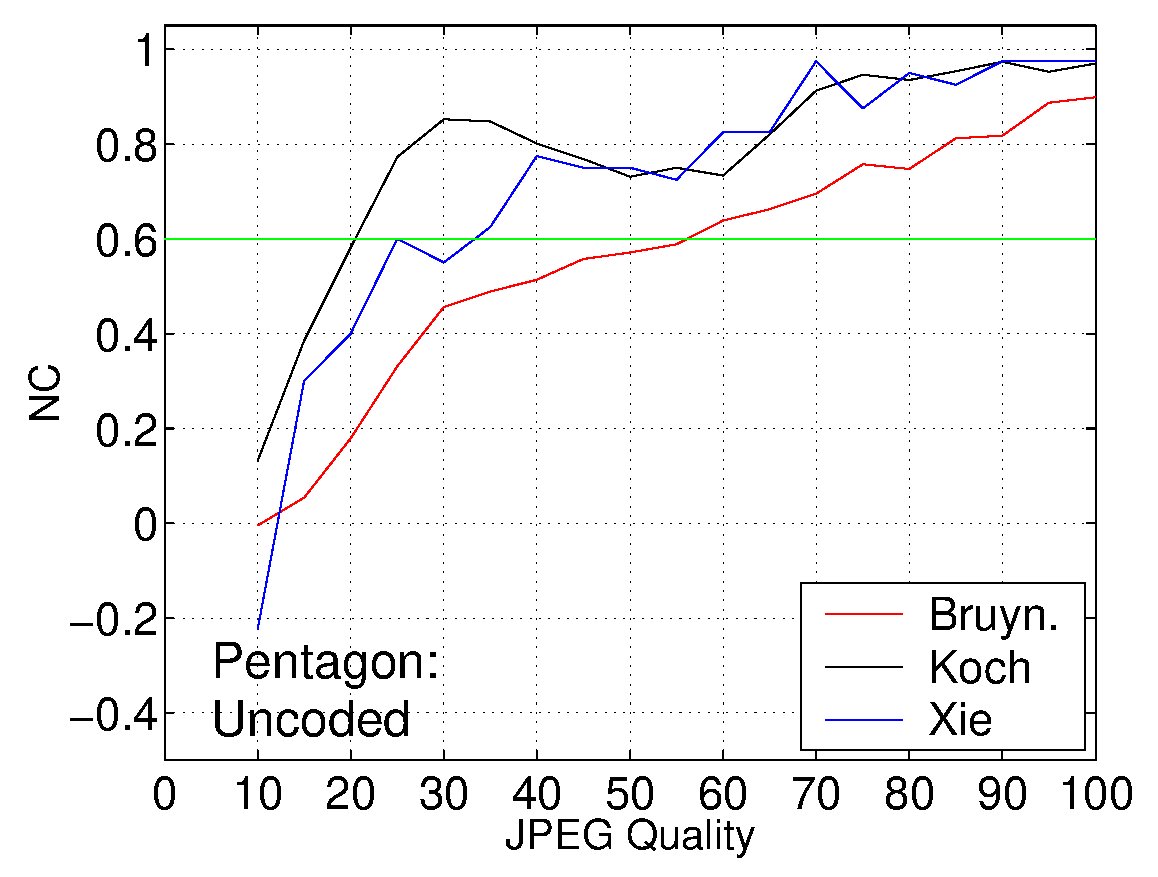
\includegraphics[height=4.6cm,width=4.8cm]{Pentagon80_80_1.eps}
        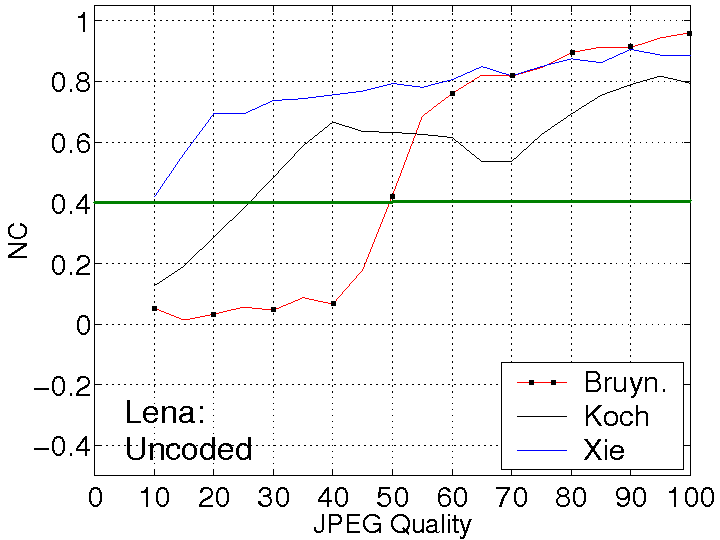
\includegraphics[height=4.5cm,width=4.5cm]{Lena320_320_1.png}
        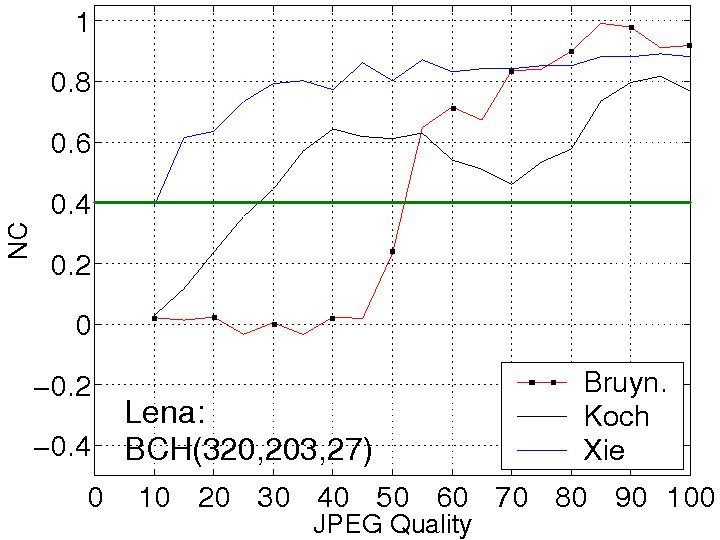
\includegraphics[height=4.5cm,width=4.5cm]{Lena320_203_27.png}
        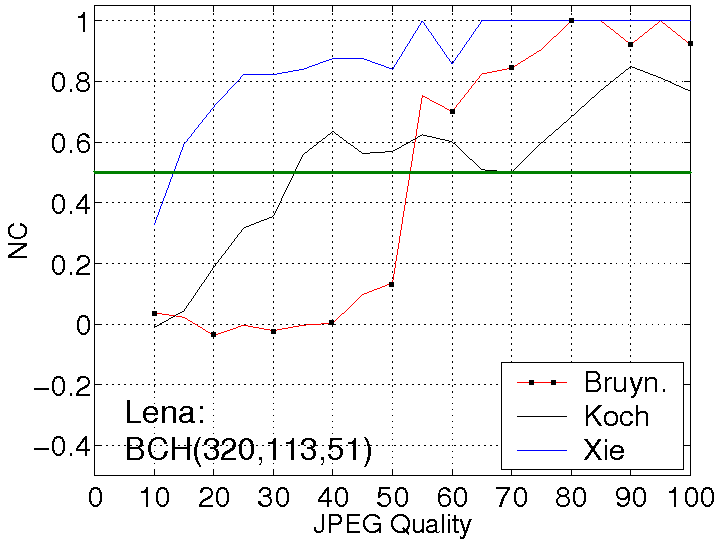
\includegraphics[height=4.5cm,width=4.5cm]{Lena320_113_51.png}
        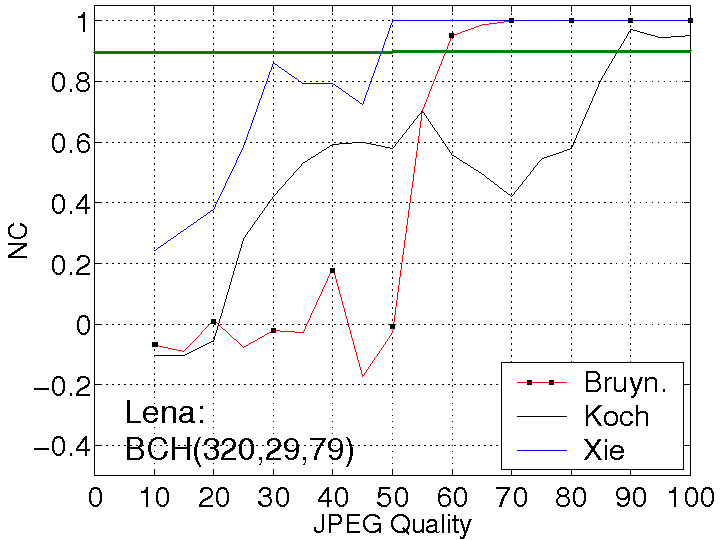
\includegraphics[height=4.5cm,width=4.5cm]{Lena320_29_79.png}
}} 
        \caption{Results for different watermarking systems using 320 bit watermarks}
        \label{fig:320BKX}
\setlength{\abovecaptionskip}{0cm}
\end{figure*}
In the {\bf Koch system}, the BCH decoded messages do not improve upon the
	uncoded message at all; the more BCH coding, the worse the performance.
In the {\bf Xie system}, it can be seen that 
BCH(320,203,27) and BCH(320,113,51) can survive strong JPEG compression attacks (similar to the 
uncoded case) yet return slightly higher NC values than the uncoded case. In particular, 
BCH(320,113,51) return perfect NC values (1.00) for all attacks down to JPEG quality 65. 
BCH(320,29,79) makes the Xie algorithm \emph{less} robust to strong JPEG attacks, but when an attack is
survived, it returns perfect NC values of 1.00. If different detector threshold values had not been used in
this analysis, a developer may wrongly conclude that 
adding any of these BCH codes to the Xie system would improve its robustness.

Analysis of the ROC values in Table~\ref{tab:rocLenaBKX} show that all three of the systems are reliable. 
In general, as more BCH code is added to any of these systems, the reliability of that system decreases.
However, as reported in Table~\ref{bkzROCBKX}, the Xie and Koch systems are more reliable (in the Lena
image) than the Bruyndonckx system. 
\begin{table}[!t]
\setlength{\abovecaptionskip}{-0.1cm}
\footnotesize
        \begin{center}
                \begin{tabular}{|c|c|c|c|c|} \hline
                Coding 			& 	& 		& 	& 	\\ 
		strategy		& Image	& Bruyndonckx   & Koch  & Xie   \\ \hline
                Uncoded         	& Lena	& 0.841         & 0.971 & 0.991 \\ \hline
                %BCH(320,257,15) 	& Lena	& 0.799         & 0.937 & 0.952 \\ \hline
                BCH(320,203,27) 	& Lena	& 0.748         & 0.925 & 0.960 \\ \hline
                %BCH(320,158,39) 	& Lena	& 0.754         & 0.926 & 0.984 \\ \hline
                BCH(320,113,51) 	& Lena	& 0.726         & 0.897 & 0.999 \\ \hline
                %BCH(320,68,61)  	& Lena	& 0.716         & 0.878 & 0.994 \\ \hline
                BCH(320,29,79)  	& Lena	& 0.717         & 0.864 & 0.909 \\ \hline
                \end{tabular}
        \end{center}
	\caption{Area under ROC graphs for 320 bit watermarks}
	%\caption{Area under ROC graphs for three different watermarking systems with 320 bit watermarks
	%under JPEG compression attack (Lena image only)}
        \label{tab:rocLenaBKX}
\end{table}
\normalsize


\section{Conclusion}
In conclusion, benchmarking tools (\emph{e.g.} NC against attack strength, 
Watson metric, detector thresholds based on fair $P_{\mathit fp}$ values,
ROC graphs and PIM)
have been used to fairly compare different watermarking systems (with and without ECCs). 
Such tools (or their equivalent) should be used by designers to compare the robustness of novel watermarking algorithms 
with existing algorithms. 
%Using all of these tools together ensures a fair analysis of a watermarking system. 
%Such methodologies should also be employed when comparing different watermarking systems (with and without ECCs)
%to give a fair and balanced analysis.

%For example,
%if the robustness of the three systems under test had been measured using only NC against attack strength graphs, it would have
%appeared as if adding BCH codes to these systems gave an increase in robustness. 
%However, when
%different detector thresholds are used (resulting in similar $P_{\mathit fp}$ values for different message lengths),
%it can be seen that adding BCH codes to these watermarking systems 
%(under the parameters used in this paper)
%%(under the conditions set out in Table~\ref{bkxVQBKX})
%results in a robustness decrease. 
%%Note that results have been obtained for other images, more signal processing attacks and different ECCs,
%%but there is enough space to analyse all of these in this paper. The results presented here introduce benchmarking tools
%%and show how they can be used to fairly compare different watermarking systems.
%%From looking at the NC against JPEG quality graphs in Figure~\ref{fig:80BKX}, it can be seen that adding BCH codes to
%%these watermarking systems results in higher NC values. However, when these graphs are analysed with fair detector threshold
%%values, it becomes clear that the uncoded systems are performing much better.
%%It was also shown that each watermarking system has a varying degree of robustness based upon the
%%complexity of the host image used to embed the watermark.
%%Analysing the ROC graphs, it could be seen that 
%%all three algorithms were reliable. 
%%It was also shown that the ROC performance of each system was image specific.
%%the transform based systems of Xie and Koch are more reliable than the spatially
%%based system of Bruyndonckx. 
%This paper aimed to introduce benchmarking tools and show how they can be used to fairly compare different watermarking systems. 


\renewcommand{\baselinestretch}{0.9}
%\scriptsize
\footnotesize
%%%%%%%%%%%%%%%%%%%%%%%%%%%%%
%%%%%%%%%%%%%%%%%%%%%%%%%%%%%
\bibliography{austria07_t4_sent_final_6pages}
\bibliographystyle{unsrt}
%\scriptsize
\footnotesize
\renewcommand{\baselinestretch}{1}

%\begin{thebibliography}{00}
%\bibitem{dugad} R. Dugad, K. Ratakonda and N. Ahuja,
%	A new wavelet-based scheme for watermarking images,
%	\emph{Proc. IEEE Intl. Conf. on Image Processing,
%	ICIP'98},
%	Chicago, IL, USA, Oct. 1998, 419-423.
%\end{thebibliography}

%%%%%%%%%%%%%%%%%%%%%%%%%%%%%%%%%%%%%%%%%%%%%%%%%%%%%%%%%%%%%%%%%%%%%%%%%%%%%%%%%%%%%%%%%%%%%%%%%%%% 

\end{document}



